\PassOptionsToPackage{table}{xcolor}
\documentclass[aspectratio=169]{beamer}

% ---------- packages ----------
\usepackage[utf8]{inputenc}
\usepackage[T1]{fontenc}
\usepackage{tikz}
\usepackage{pgfplots}
\pgfplotsset{compat=1.18}
\usepackage{colortbl}
\usepackage{amssymb}
\usepackage{overpic}
\usetikzlibrary{arrows.meta,positioning,shapes.geometric,fit}

% ---------- palette (professional light theme) ----------
\definecolor{pvnavy}{HTML}{1F3A5F}
\definecolor{pvbg}{HTML}{FFFFFF}
\definecolor{pvsurface}{HTML}{EEF2F7}
\definecolor{pvborder}{HTML}{C9D3E0}
\definecolor{pvtext}{HTML}{2B2B2B}
\definecolor{pvbright}{HTML}{1F3A5F}
\definecolor{pvaccent}{HTML}{1F3A5F}
\definecolor{pvhl}{HTML}{F5B301}   % highlight for annotations on dark spectrograms
\definecolor{pvsub}{HTML}{FFFFFF}

\usetheme{Madrid}
\usecolortheme{default}
\usefonttheme{professionalfonts}
\setbeamercolor{structure}{fg=pvnavy}
\setbeamercolor{palette primary}{bg=pvnavy,fg=white}
\setbeamercolor{palette secondary}{bg=pvnavy!85!black,fg=white}
\setbeamercolor{palette tertiary}{bg=pvnavy!70!black,fg=white}
\setbeamercolor{title}{bg=pvnavy,fg=white}
\setbeamercolor{frametitle}{bg=pvnavy,fg=white}
\setbeamercolor{framesubtitle}{fg=white!85!pvnavy}
\setbeamercolor{normal text}{fg=pvtext,bg=white}
\setbeamercolor{block title}{bg=pvnavy,fg=white}
\setbeamercolor{block body}{bg=pvsurface,fg=pvtext}
\setbeamercolor{item}{fg=pvnavy}
\setbeamertemplate{blocks}[rounded][shadow=false]
\setbeamertemplate{navigation symbols}{}
\setbeamertemplate{footline}{%
  \leavevmode\hbox{%
  \begin{beamercolorbox}[wd=.5\paperwidth,ht=2.4ex,dp=1ex,left,leftskip=1em]{palette primary}%
    \usebeamerfont{footline}\insertshorttitle
  \end{beamercolorbox}%
  \begin{beamercolorbox}[wd=.5\paperwidth,ht=2.4ex,dp=1ex,right,rightskip=1em]{palette secondary}%
    \usebeamerfont{footline}\insertshortinstitute\hspace{2em}\insertframenumber{} / \inserttotalframenumber
  \end{beamercolorbox}}%
  \vskip0pt}
\arrayrulecolor{pvborder}
\renewcommand{\arraystretch}{1.25}

% ---------- reusable tikz styles ----------
\tikzstyle{pvbox}=[draw=pvnavy,fill=pvsurface,text=pvnavy,rounded corners,thick,
  minimum height=0.9cm,minimum width=2.6cm,align=center,font=\small,inner sep=4pt]
\tikzstyle{pvarrow}=[-{Latex[length=2mm]},draw=pvtext,thick]
\tikzstyle{pvstage}=[draw=pvnavy,fill=pvnavy,text=white,rounded corners,thick,
  minimum height=0.75cm,minimum width=3.0cm,align=center,font=\small\bfseries,inner sep=3pt]
\tikzstyle{pvstep}=[draw=pvnavy,fill=pvsurface,text=pvtext,rounded corners=2pt,
  minimum height=0.55cm,text width=2.9cm,align=center,font=\scriptsize,inner sep=2pt]
\tikzstyle{pvgroup}=[draw=pvnavy!60,dashed,rounded corners,inner sep=6pt]
\pgfmathdeclarefunction{sinc}{1}{\pgfmathparse{(#1==0)?1:sin(#1*180/pi)/#1}}

\title[Phase Vocoder Voice Changer]{Phase Vocoder Voice Changer}
\subtitle{Independent speed \& pitch control for speech, with transient preservation}
\institute[CSE220]{CSE220 --- Signals and Systems}
\date{}

\begin{document}

\begin{frame}
  \titlepage
\end{frame}

% ======================================================================
\section{Problem}
\begin{frame}{The Problem}
  \begin{block}{Speed and pitch are physically glued together}
    On a computer, playing a signal faster or slower is the same operation
    as changing its sample rate --- so pitch moves with it, whether you
    want it to or not.
  \end{block}
  \vspace{0.3cm}
  \begin{itemize}
    \item Speed up naively $\rightarrow$ pitch goes \textbf{up} (chipmunk effect).
    \item Slow down naively $\rightarrow$ pitch goes \textbf{down} (drone/slow-motion effect).
    \item Almost nobody actually wants that coupling --- they want \emph{one}
      knob, not both moving together.
  \end{itemize}
  \vspace{0.3cm}
  \centering{\large\color{pvaccent} That coupling is exactly what this project removes.}
\end{frame}

% ======================================================================
\section{What It Does}
\begin{frame}{What Our Software Does}
  \begin{columns}[T,onlytextwidth]
    \column{0.32\textwidth}
      
\begin{tikzpicture}
        \node[pvbox,minimum height=2.2cm,minimum width=\linewidth] (a) {%
          \Large\textbf{Speed}\\[4pt]\normalsize 0.25$\times$--2.4$\times$\\ independent of pitch};
      \end{tikzpicture}
    \column{0.32\textwidth}
      
\begin{tikzpicture}
        \node[pvbox,minimum height=2.2cm,minimum width=\linewidth] (b) {%
          \Large\textbf{Pitch}\\[4pt]\normalsize $\pm$3--12 semitones\\ independent of speed};
      \end{tikzpicture}
    \column{0.32\textwidth}
      
\begin{tikzpicture}
        \node[pvbox,minimum height=2.2cm,minimum width=\linewidth] (c) {%
          \Large\textbf{Transients}\\[4pt]\normalsize consonants stay\\ sharp, not smeared};
      \end{tikzpicture}
  \end{columns}
  \vspace{0.5cm}
  \begin{itemize}
    \item Input: any file \texttt{soundfile}/FFmpeg can decode (WAV, MP3, FLAC, OGG), or a live mic recording.
    \item Two quality/cost modes: \textbf{Fast} (cheap, small pitch shifts) and
      \textbf{Accurate} (resample + stretch, wider range).
    \item A built-in \textbf{naive-resample} comparison mode, to demonstrate the
      problem this solves.
  \end{itemize}
\end{frame}

% ======================================================================
\section{Spotting the Change}
\begin{frame}{Spotting the Change --- How to Read the Result}
  \framesubtitle{Pitch shift down: $-9$ semitones, speed $1.0\times$ (Accurate mode)}
  \begin{columns}[T,onlytextwidth]
    \column{0.63\textwidth}
      \begin{tikzpicture}
        \node[anchor=south west,inner sep=0] (img) at (0,0)
          {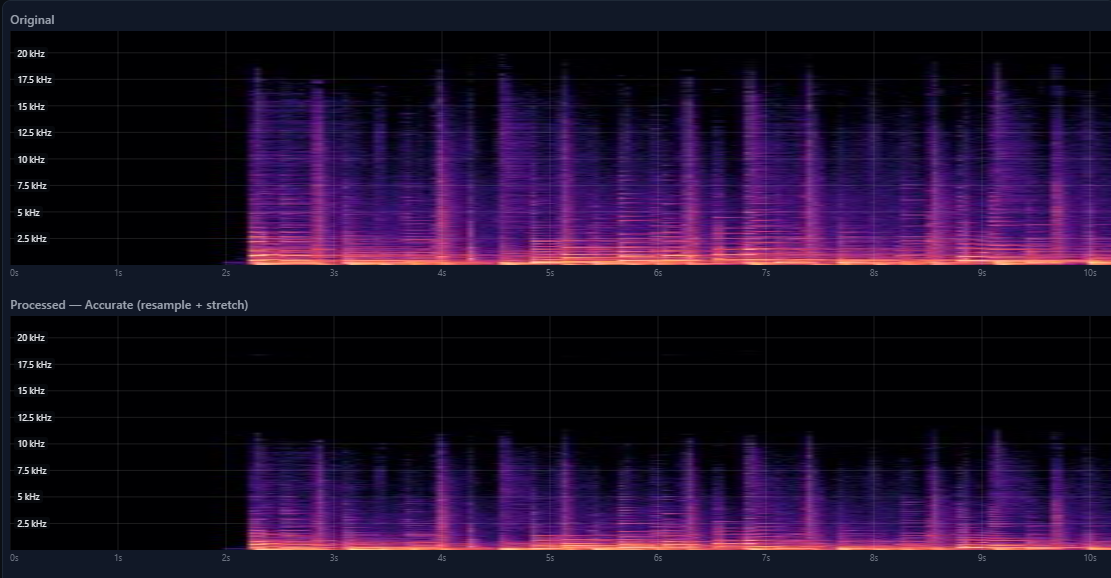
\includegraphics[width=\linewidth]{img_pitch_only.png}};
        \begin{scope}[x={(img.south east)},y={(img.north west)}]
          % top panel: original energy ceiling (~19 kHz)
          \draw[pvhl,thick,dashed] (0.21,0.888) -- (0.99,0.888);
          \node[pvhl,font=\tiny\bfseries,anchor=south east] at (0.99,0.889) {top of voice energy $\approx$ 19 kHz};
          % bottom panel: where it was vs. where it is now
          \draw[pvhl!60,thin,dashed] (0.21,0.398) -- (0.99,0.398);
          \draw[pvhl,thick,dashed] (0.21,0.247) -- (0.99,0.247);
          \draw[-{Latex[length=1.6mm]},pvhl,very thick] (0.60,0.395) -- (0.60,0.255);
          \node[pvhl,font=\tiny\bfseries,anchor=west] at (0.61,0.325) {drops to $\approx$ 11 kHz};
          % same onset times in both panels
          \draw[white,thick,densely dotted] (0.223,0.03) -- (0.223,0.955);
          \draw[white,thick,densely dotted] (0.396,0.03) -- (0.396,0.955);
          \node[white,font=\tiny\bfseries,fill=black,fill opacity=0.6,text opacity=1,inner sep=1pt,anchor=north]
            at (0.31,0.52) {same timing};
        \end{scope}
      \end{tikzpicture}
    \column{0.34\textwidth}
      \scriptsize
      \textbf{How to read a spectrogram}
      \begin{itemize}\scriptsize
        \item $x$-axis = time, $y$-axis = frequency, brightness = energy.
        \item Horizontal bands = harmonics (pitch of vowels).
        \item Vertical streaks = transients (consonant onsets).
      \end{itemize}
      \vspace{2pt}
      \textbf{What changed}
      \begin{itemize}\scriptsize
        \item Top = original, bottom = our output.
        \item Every band moves \textbf{down} by the same ratio:
          $2^{-9/12}\approx0.59$, so $19\,\text{kHz}\times0.59\approx11\,\text{kHz}$.
        \item Onsets (dotted lines) stay at the \textbf{same seconds} --- the clip
          length is unchanged.
      \end{itemize}
      \vspace{2pt}
      {\color{pvnavy}\textbf{Pitch moved, time did not.}}
  \end{columns}
\end{frame}

% ======================================================================
\section{Pipeline}
\begin{frame}{Solution Overview: The Pipeline}
  \centering
  \resizebox{\linewidth}{!}{%
  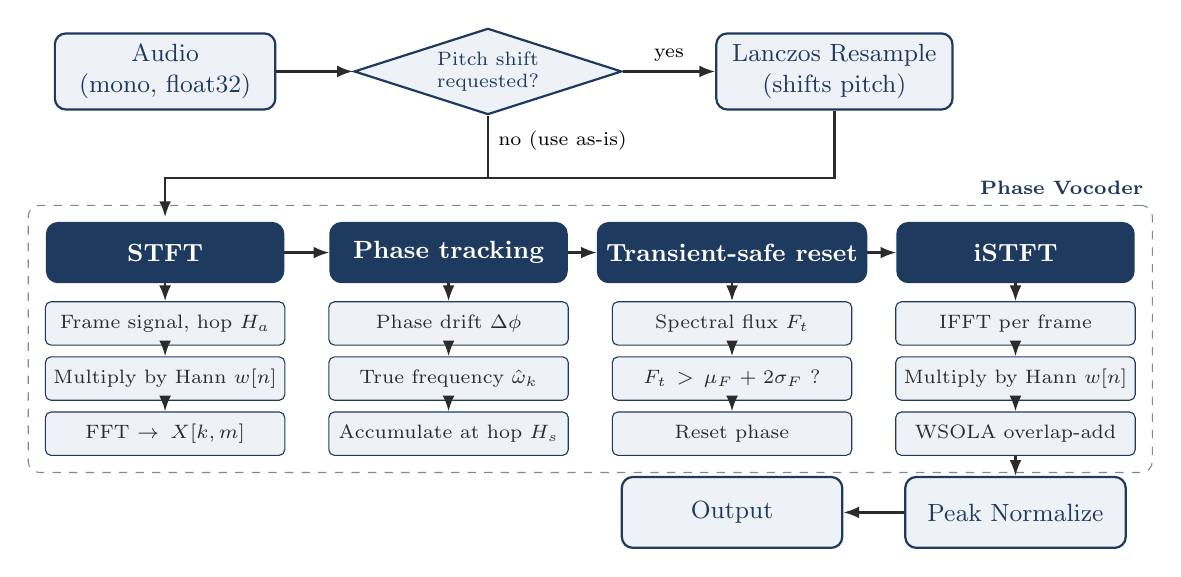
\begin{tikzpicture}[every node/.style={font=\small}]
    % ---- pre-processing ----
    \node[pvbox,minimum width=2.8cm] (audio) at (1.5,0) {Audio\\(mono, float32)};
    \node[diamond,draw=pvnavy,thick,fill=pvsurface,text=pvnavy,aspect=2.6,align=center,
          minimum width=3.4cm,font=\scriptsize,inner sep=1pt] (dec) at (5.6,0) {Pitch shift\\requested?};
    \node[pvbox,minimum width=3.0cm] (res) at (10.0,0) {Lanczos Resample\\(shifts pitch)};
    \draw[pvarrow] (audio) -- (dec);
    \draw[pvarrow] (dec) -- node[above,font=\scriptsize]{yes} (res);
    \coordinate (merge) at (1.5,-1.35);
    \draw[pvarrow] (dec.south) -- node[right,font=\scriptsize,pos=0.4]{no (use as-is)} (5.6,-1.35) -- (merge) -- (1.5,-1.85);
    \draw[thick,draw=pvtext] (res.south) -- (10.0,-1.35) -- (5.6,-1.35);

    % ---- phase vocoder: four stages ----
    \node[pvstage] (stft) at (1.5,-2.3)  {STFT};
    \node[pvstage] (pt)   at (5.1,-2.3)  {Phase tracking};
    \node[pvstage] (tr)   at (8.7,-2.3)  {Transient-safe reset};
    \node[pvstage] (istft)at (12.3,-2.3) {iSTFT};
    \draw[pvarrow] (stft) -- (pt);
    \draw[pvarrow] (pt) -- (tr);
    \draw[pvarrow] (tr) -- (istft);

    % STFT steps
    \node[pvstep] (s1) at (1.5,-3.2) {Frame signal, hop $H_a$};
    \node[pvstep] (s2) at (1.5,-3.9)  {Multiply by Hann $w[n]$};
    \node[pvstep] (s3) at (1.5,-4.6) {FFT $\rightarrow X[k,m]$};
    \draw[pvarrow] (s1) -- (s2); \draw[pvarrow] (s2) -- (s3);
    % phase tracking steps
    \node[pvstep] (p1) at (5.1,-3.2) {Phase drift $\Delta\phi$};
    \node[pvstep] (p2) at (5.1,-3.9)  {True frequency $\hat\omega_k$};
    \node[pvstep] (p3) at (5.1,-4.6) {Accumulate at hop $H_s$};
    \draw[pvarrow] (p1) -- (p2); \draw[pvarrow] (p2) -- (p3);
    % transient steps
    \node[pvstep] (t1) at (8.7,-3.2) {Spectral flux $F_t$};
    \node[pvstep] (t2) at (8.7,-3.9)  {$F_t>\mu_F+2\sigma_F$ ?};
    \node[pvstep] (t3) at (8.7,-4.6) {Reset phase};
    \draw[pvarrow] (t1) -- (t2); \draw[pvarrow] (t2) -- (t3);
    % iSTFT steps
    \node[pvstep] (i1) at (12.3,-3.2) {IFFT per frame};
    \node[pvstep] (i2) at (12.3,-3.9)  {Multiply by Hann $w[n]$};
    \node[pvstep] (i3) at (12.3,-4.6) {WSOLA overlap-add};
    \draw[pvarrow] (i1) -- (i2); \draw[pvarrow] (i2) -- (i3);

    \foreach \a/\b in {stft/s1,pt/p1,tr/t1,istft/i1} {\draw[pvarrow] (\a) -- (\b);}

    \node[pvgroup,fit=(stft)(istft)(s3)(i3)] (grp) {};
    \node[anchor=south east,font=\scriptsize\bfseries,text=pvnavy] at (grp.north east) {Phase Vocoder};

    % ---- output ----
    \node[pvbox,minimum width=2.8cm] (norm) at (12.3,-5.6) {Peak Normalize};
    \node[pvbox,minimum width=2.8cm] (out)  at (8.7,-5.6)  {Output};
    \draw[pvarrow] (i3) -- (norm);
    \draw[pvarrow] (norm) -- (out);
  \end{tikzpicture}}
\end{frame}

% ======================================================================
\section{Processing Stages (Backup)}
\begin{frame}{Stage 1: Audio Loading}
  \framesubtitle{Backup --- for Q\&A}
  \begin{columns}[T]
    \column{0.5\textwidth}
      \textbf{Input:} any decodable audio file or mic recording.\\[4pt]
      \textbf{Output:} 1-D mono \texttt{float32}, range $[-1,1]$, native sample rate.\\[4pt]
      \textbf{Algorithm:} read via \texttt{soundfile}; down-mix multi-channel by averaging.
    \column{0.5\textwidth}
      \[ x_{\text{mono}}[n] = \frac{1}{C}\sum_{c=1}^{C} x_c[n] \]
      \small\textbf{Why:} every later stage assumes one real 1-D signal.\\[6pt]
      \small\textbf{Viva note:} stereo width is permanently lost here (known limitation).
  \end{columns}
\end{frame}

\begin{frame}{Stage 2: STFT}
  \framesubtitle{Backup --- for Q\&A}
  \textbf{Input:} mono waveform. \quad \textbf{Output:} complex matrix $X[k,m]$ (freq.\ bin $\times$ frame).\\[4pt]
  \textbf{Steps:} (1) cut overlapping frames, hop $H_a$ \; (2) multiply each frame by the Hann window \; (3) FFT each frame.
  \[ X[k,m] = \sum_{n=0}^{N-1} x[mR+n]\,w[n]\,e^{-j\frac{2\pi}{N}kn} \]
  \centering
  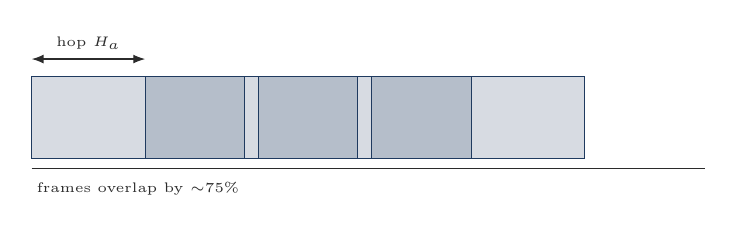
\begin{tikzpicture}[scale=0.9]
    \draw[pvtext] (0,0) -- (9.5,0);
    \foreach \i in {0,1,2,3} {
      \draw[draw=pvaccent,fill=pvaccent,fill opacity=0.18] (\i*1.6,0.15) rectangle (\i*1.6+3,1.3);
    }
    \draw[{Latex[length=1.5mm]}-{Latex[length=1.5mm]},pvtext] (0,1.55) -- (1.6,1.55)
      node[midway,above,font=\tiny]{hop $H_a$};
    \node[font=\tiny,anchor=north,pvtext] at (1.5,-0.05) {frames overlap by $\sim$75\%};
  \end{tikzpicture}
\end{frame}

\begin{frame}{Stage 3: Phase Vocoder}
  \framesubtitle{Backup --- for Q\&A}
  \textbf{Input:} STFT matrix, target speed factor, optional pitch factor.\\
  \textbf{Output:} phase-corrected spectrum, re-hopped at synthesis spacing $H_s$.\\[4pt]
  \textbf{Algorithm:} estimate true instantaneous frequency per bin from phase drift, re-accumulate phase at $H_s$.
  \[ \hat\omega_k = \omega_k + \frac{\Delta\phi-\omega_k H_a}{H_a}, \qquad
     \phi_{\text{out}}[m]=\phi_{\text{out}}[m-1]+\hat\omega_k H_s \]
  \centering
  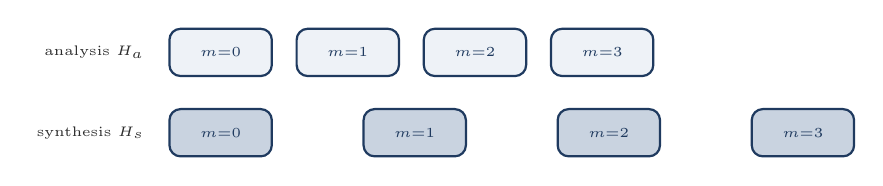
\begin{tikzpicture}[scale=0.85]
    \foreach \i in {0,1,2,3} {\node[pvbox,minimum width=1.3cm,minimum height=0.6cm,font=\tiny] at (\i*1.9,1.2) {$m$=\i};}
    \foreach \i in {0,1,2,3} {\node[pvbox,minimum width=1.3cm,minimum height=0.6cm,font=\tiny,fill=pvborder] at (\i*2.9,0) {$m$=\i};}
    \node[font=\tiny,anchor=east,pvtext] at (-1.0,1.2) {analysis $H_a$};
    \node[font=\tiny,anchor=east,pvtext] at (-1.0,0) {synthesis $H_s$};
  \end{tikzpicture}
\end{frame}

\begin{frame}{Stage 4: Transient Detection \& Phase Reset}
  \framesubtitle{Backup --- for Q\&A}
  \textbf{Input:} STFT magnitude $|X[k,m]|$. \quad
  \textbf{Output:} per-frame transient flag; phase reset instead of accumulated on that frame.\\[4pt]
  \textbf{Algorithm:} spectral flux vs.\ an adaptive threshold from recent history.
  \[ F_t=\sum_k \max(0,|X_t(k)|-|X_{t-1}(k)|), \qquad \text{transient if } F_t > \mu_F+2\sigma_F \]
  \centering
  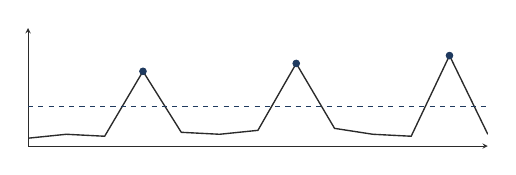
\begin{tikzpicture}[scale=0.62]
    \begin{axis}[width=11cm,height=4cm,axis lines=left,
      xtick=\empty,ytick=\empty,ymin=0,ymax=6,
      axis line style={pvtext},
      tick label style={pvtext}]
      \addplot[pvtext,thick] coordinates {(0,0.4)(1,0.6)(2,0.5)(3,3.8)(4,0.7)(5,0.6)(6,0.8)(7,4.2)(8,0.9)(9,0.6)(10,0.5)(11,4.6)(12,0.6)};
      \addplot[pvaccent,dashed,thick] coordinates {(0,2)(12,2)};
      \addplot[only marks,mark=*,mark options={fill=pvaccent,draw=pvaccent}] coordinates {(3,3.8)(7,4.2)(11,4.6)};
    \end{axis}
  \end{tikzpicture}
  \small (schematic) dashed line = adaptive threshold $\mu_F+2\sigma_F$; dots = phase-reset frames.
\end{frame}

\begin{frame}{Stage 5: Lanczos Resampling}
  \framesubtitle{Backup --- for Q\&A}
  \textbf{Input:} audio, stretch factor $s$. \quad \textbf{Output:} signal of length $N\!\cdot\! s$.\\[4pt]
  \textbf{Algorithm:} windowed-sinc interpolation; cutoff lowers to new Nyquist when compressing ($s<1$).
  \[ r=\min(1,s), \qquad L_a(x)=r\cdot\mathrm{sinc}(rx)\cdot\mathrm{sinc}(rx/a) \]
  \centering
  \begin{tikzpicture}[scale=0.62]
    \begin{axis}[width=11cm,height=4cm,axis lines=middle,
      xtick=\empty,ytick=\empty,ymin=-0.3,ymax=1.1,
      axis line style={pvtext}]
      \addplot[pvaccent,thick,samples=300,domain=-11.9:11.9] {sinc(x)*sinc(x/8)};
    \end{axis}
  \end{tikzpicture}
  \small $a=8$ taps by default --- same operation used for the naive-resample comparison clip, minus the phase-vocoder correction step.
\end{frame}

\begin{frame}{Stage 6: Final Output}
  \framesubtitle{Backup --- for Q\&A}
  \textbf{Input:} reconstructed audio from overlap-add. \quad
  \textbf{Output:} peak-normalized \texttt{float32} audio; Accurate mode also writes a WAV.\\[4pt]
  \textbf{Steps (iSTFT):} (1) IFFT each frame \; (2) multiply by the Hann window \; (3) WSOLA overlap-add at hop $H_s$, then scale by loudest sample.
  \[ y[n]=\frac{\sum_m y_m[n-mR]\,w[n-mR]}{\sum_m w^2[n-mR]}, \qquad
     x_{\text{norm}}=\frac{x}{\max|x|}\times0.99 \]
  \small\textbf{Viva note:} at identity settings (speed 1.0, shift 0) the app reports a round-trip SNR --- a sanity check, not a general quality metric.
\end{frame}

% ======================================================================
\section{Trade-offs}
\begin{frame}{Trade-offs: Window Size, Overlap \& Limits}
  \centering
  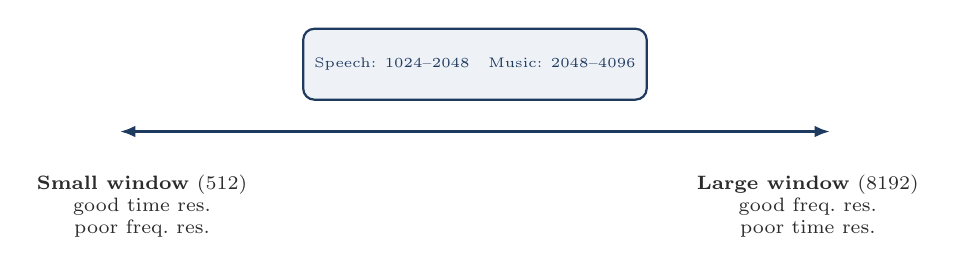
\begin{tikzpicture}[scale=0.95]
    \draw[{Latex[length=2mm]}-{Latex[length=2mm]},pvaccent,very thick] (0,0) -- (9.5,0);
    \node[align=center,font=\scriptsize,text=pvtext] at (0.3,-1.0) {\textbf{Small window} (512)\\good time res.\\poor freq.\ res.};
    \node[align=center,font=\scriptsize,text=pvtext] at (9.2,-1.0) {\textbf{Large window} (8192)\\good freq.\ res.\\poor time res.};
    \node[pvbox,font=\tiny] at (4.75,0.9) {Speech: 1024--2048\quad Music: 2048--4096};
  \end{tikzpicture}
  \vspace{0.4cm}
  \small
  \begin{itemize}
    \item Overlap rises with $|\text{effective stretch}-1|$: \textbf{75\%} default $\to$ up to \textbf{90\%} for extreme stretch.
    \item Hard limit (code-enforced): compound time-stretch $\mathbf{0.25\times}$--$\mathbf{3.0\times}$.
    \item Pitch shift: $\pm3$ st (Fast mode) / $\pm12$ st (Accurate mode); artifacts grow past $\sim\pm9$.
    \item Playback speed (UI): $0.25\times$--$2.4\times$.
  \end{itemize}
\end{frame}

\begin{frame}{Transient Preservation}
  \textbf{Problem:} accumulating phase through a consonant onset smears it into neighboring frames.\\[4pt]
  \textbf{Fix:} detect the onset via spectral flux, then \textbf{reset} synthesis phase to the analysis phase at that frame --- resume normal accumulation right after.\\[6pt]
  \[ F_t=\sum_k\max(0,|X_t(k)|-|X_{t-1}(k)|) \]
  \small A short $\sim$20\,ms refractory window stops one long attack from re-triggering every frame it spans.
\end{frame}

\begin{frame}{Resampling: Why Not Just Interpolate Linearly?}
  \begin{itemize}
    \item Linear interpolation has \textbf{no anti-aliasing} --- compressing a
      signal folds high frequencies back into the audible range as metallic,
      comb-like artifacts.
    \item Lanczos (windowed-sinc) resampling has a built-in low-pass cutoff
      when compressing, so it filters as it resamples.
    \item Trade-off: more computation per sample (wider kernel) for a clean result.
  \end{itemize}
  \vspace{0.3cm}
  \centering\color{pvaccent}\large ``Linear resampling aliases; Lanczos filters as it resamples.''
\end{frame}

% ======================================================================
\section{Results}
\begin{frame}{Result: Speed-Only Change (2$\times$, Fast mode)}
  \centering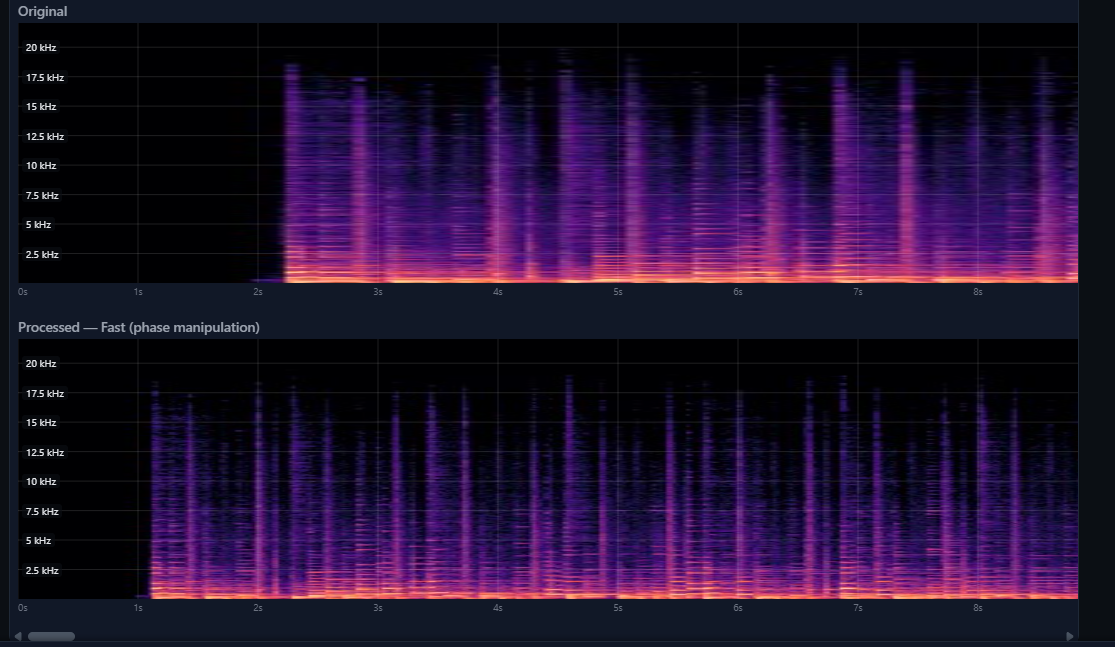
\includegraphics[width=\linewidth,height=0.7\textheight,keepaspectratio]{img_speed_only.png}\par
  \small Semitone shift = 0. Notice the harmonic bands stay at the same
  height while the clip compresses in time --- speed changed, pitch did not.
\end{frame}

\begin{frame}{Result: Pitch-Only Change ($-9$ semitones, Accurate mode)}
  \centering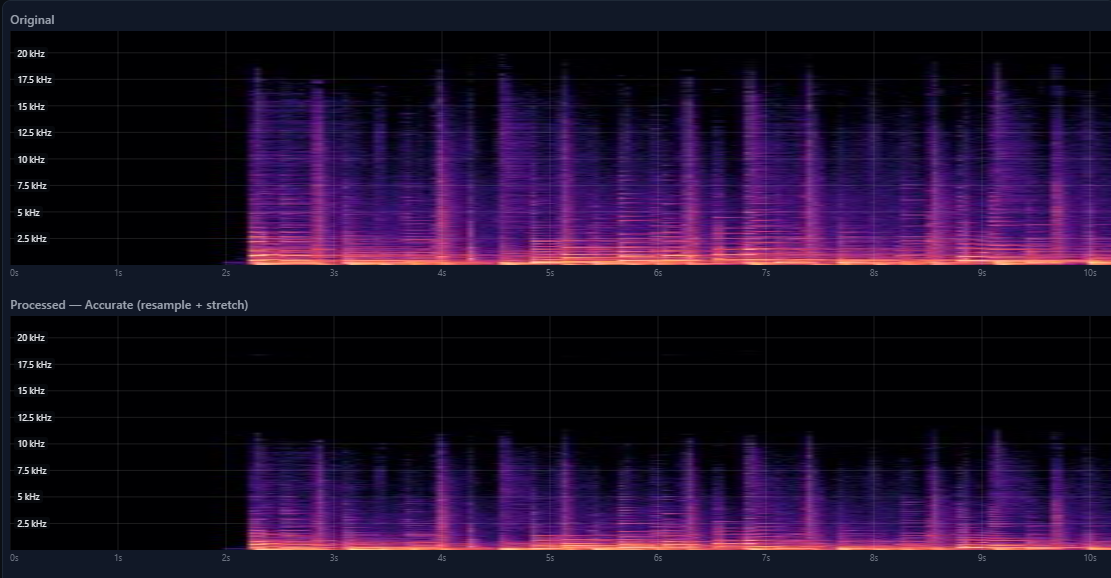
\includegraphics[width=\linewidth,height=0.7\textheight,keepaspectratio]{img_pitch_only.png}\par
  \small Speed factor = 1.0. Notice the harmonic bands drop to a lower
  frequency while the timeline is unchanged --- pitch changed, duration did not.
\end{frame}

\begin{frame}{Result: Naive vs.\ Accurate --- 2$\times$ Speed-Up}
  \centering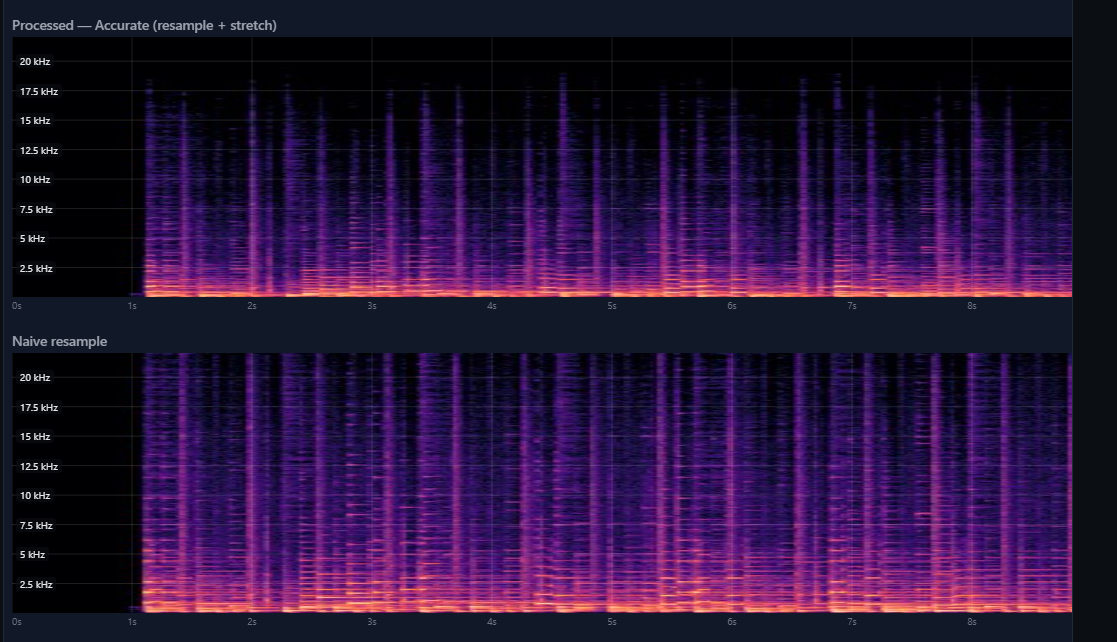
\includegraphics[width=\linewidth,height=0.7\textheight,keepaspectratio]{img_naive_2x.png}\par
  \small Same target duration, two methods. Naive resample's bands rise with
  the speed-up; our output's bands stay put.
\end{frame}

\begin{frame}{Result: Naive vs.\ Accurate --- 0.5$\times$ Speed (Slow-Down)}
  \centering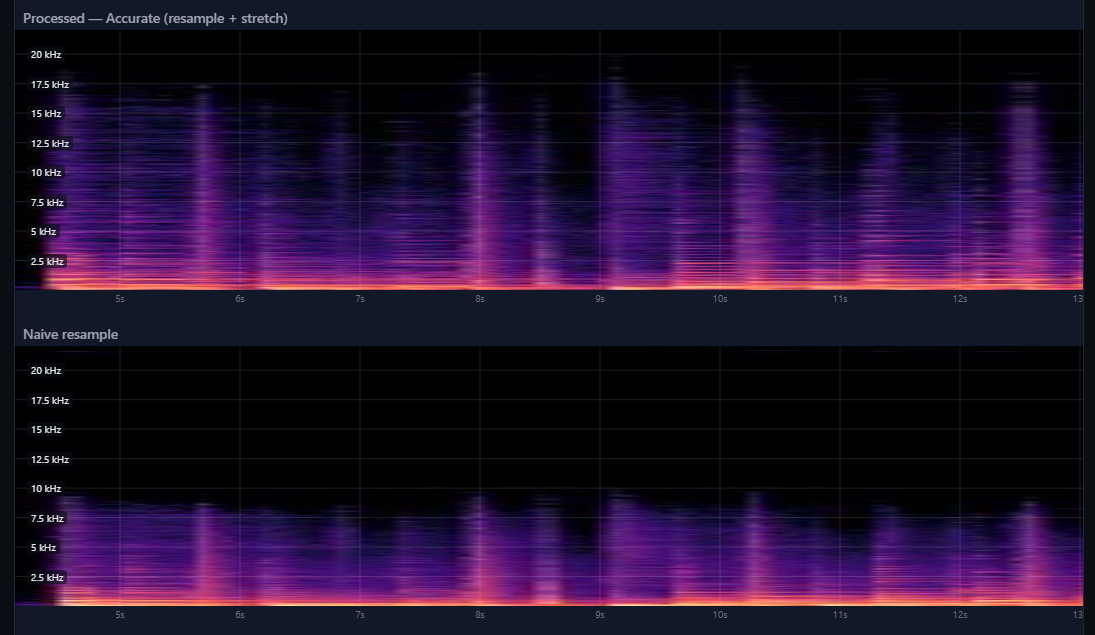
\includegraphics[width=\linewidth,height=0.7\textheight,keepaspectratio]{img_naive_half.png}\par
  \small Same slow-down, two methods. Naive resample's bands drop as the
  clip is stretched; our output again keeps them fixed.
\end{frame}

% ======================================================================
\section{Evaluation}
\begin{frame}{Evaluation Checklist}
  \centering
  \begin{tabular}{lc}
    \hline
    \textbf{Feature} & \textbf{Implemented} \\
    \hline
    Speed control & \checkmark \\
    Pitch shift & \checkmark \\
    Independent speed/pitch control & \checkmark \small(within $0.25$--$3.0\times$ effective stretch) \\
    Transient preservation (speech) & \checkmark \\
    Naive-resample comparison mode & \checkmark \\
    Formant preservation & $\times$ \\
    Stereo support & $\times$ \small(mono only, down-mixed on load) \\
    \hline
  \end{tabular}
  \vspace{0.4cm}\\
  \small\textit{Stated up front, not hidden: mono-only, no formant correction --- both are
  known scope limits, not missing features we forgot.}
\end{frame}

% ======================================================================
\section{Conclusion}
\begin{frame}{Conclusion}
  \begin{itemize}
    \item Speed and pitch, unglued --- with a transient-aware phase vocoder
      keeping speech intelligible.
    \item Two black-box algorithms doing the heavy lifting: \textbf{phase
      vocoder} for time, \textbf{Lanczos resampling} for pitch.
    \item Fast and Accurate modes trade cost for pitch-shift range.
  \end{itemize}
  \vspace{0.5cm}
  \centering\Large\color{pvaccent} Questions?
\end{frame}

% ======================================================================
\appendix
\section*{Appendix --- Viva Backup}
\begin{frame}{Appendix: STFT Overlap-Add / WOLA Normalization}
  Overlap-adding windowed frames reintroduces the window's amplitude ripple.
  Dividing by the running sum of \emph{squared} windows at each sample
  position removes it --- for Hanning + 75\% overlap this sum is nearly
  constant, so the correction is small.
\end{frame}

\begin{frame}{Appendix: Phase Accumulation}
  Replaying analysis phase directly at a new hop breaks phase continuity
  between frames (heard as warbling). Re-accumulating from the
  \emph{estimated instantaneous frequency} instead keeps phase continuous
  across the new hop spacing.
\end{frame}

\begin{frame}{Appendix: Why Hann (Hanning) Window}
  Tapers to exactly zero at both endpoints, suppressing the spectral
  leakage a hard rectangular edge would introduce. With 75\% overlap its
  squared-sum is nearly constant --- the standard choice for WOLA.
  Implemented by hand: $w[n]=0.5(1-\cos(2\pi n/(N-1)))$.
\end{frame}

\begin{frame}{Appendix: Why Lanczos (Not a Simpler Kernel)}
  A plain truncated sinc still has large sidelobes. Lanczos windows the
  sinc with \emph{another} sinc, giving a sharper frequency-domain rolloff
  for a similar tap count --- that rolloff is what supplies anti-aliasing
  when compressing.
\end{frame}

\begin{frame}{Appendix: Spectral-Flux Threshold Choice}
  Threshold $=\mu_F+2\sigma_F$ over the trailing $\sim$250\,ms of frames
  (current frame excluded, so a spike can't inflate its own threshold).
  Two standard deviations is a common "clearly above noise floor"
  heuristic --- not derived from a formal false-positive budget here.
\end{frame}

\begin{frame}{Appendix: Adaptive Threshold, Not a Fixed Gaussian $\sigma$}
  The mean/$\sigma$ above are recomputed every frame from a
  \emph{sliding window} of recent flux values --- the threshold adapts to
  the clip's current energy level rather than using one fixed number for
  the whole track.
\end{frame}

\begin{frame}{Appendix: Phase Reset Mechanics}
  On a flagged transient frame, the synthesis phase is simply set to that
  frame's own analysis phase, bypassing the accumulation recurrence for
  one frame only; accumulation resumes normally on the next frame.
\end{frame}

\begin{frame}{Appendix: Computational Complexity}
  Dominant cost: $O(N\log N)$ FFT/IFFT per frame $\times$ number of frames
  ($\approx$ signal length / hop size). Smaller hop (higher overlap) means
  more frames; the Lanczos resampler is chunked ($250{,}000$ samples/chunk)
  to keep memory bounded on long clips.
\end{frame}

\begin{frame}{Appendix: Valid Range \& Why It's a Hard Wall}
  The implementation raises an error outside $0.25\times$--$3.0\times$
  effective stretch --- a deliberate refuse-rather-than-degrade choice,
  since phase-tracking quality falls off in a way that's hard to bound
  gracefully near the edges.
\end{frame}

\end{document}
